% ==================== 2.4.1 反演中心 ====================
\subsubsection{反演中心（\texorpdfstring{$P\,\bar1$}{P-1}）}

反演中心（对称中心）$\bar1$ 是一个几何点，操作前后两原子位于同一直线上、关于该点
等距反向。为观察反演操作，选用对称性最低的中心对称空间群 $P\,\bar1$（No.~2，三斜
晶系），晶胞中只输入一个 Si 原子，建模参数见表~\ref{tab:sym-inv}。

\begin{table}[H]
  \centering
  \caption{反演中心演示的建模参数}
  \label{tab:sym-inv}
  \begin{tabular}{ll}
    \toprule
    项目 & 参数 \\
    \midrule
    空间群 & $P\,\bar1$（No.~2，三斜晶系） \\
    晶格常数 & $a=b=c=2.0$\,\AA，$\alpha=\beta=90^\circ$，$\gamma=120^\circ$ \\
    原子坐标 & Si：$(0.2,\,0.3,\,0.4)$（一般位置） \\
    等效位置数 & 2（单胞内 2 个原子） \\
    \bottomrule
  \end{tabular}
\end{table}

\begin{figure}[H]
  \centering
  \subcaptionbox{(a) 空间群与晶胞参数设置}{%
    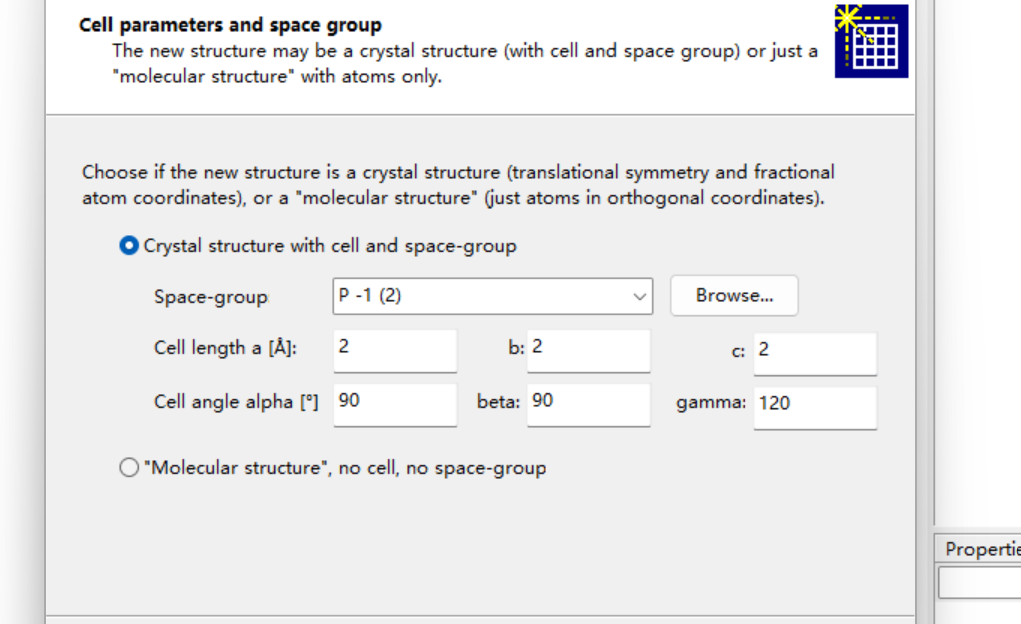
\includegraphics[width=0.44\textwidth]{assets/symmetry/inversion/a.png}}
  \hfill
  \subcaptionbox{(b) 非对称单元原子（Si）添加}{%
    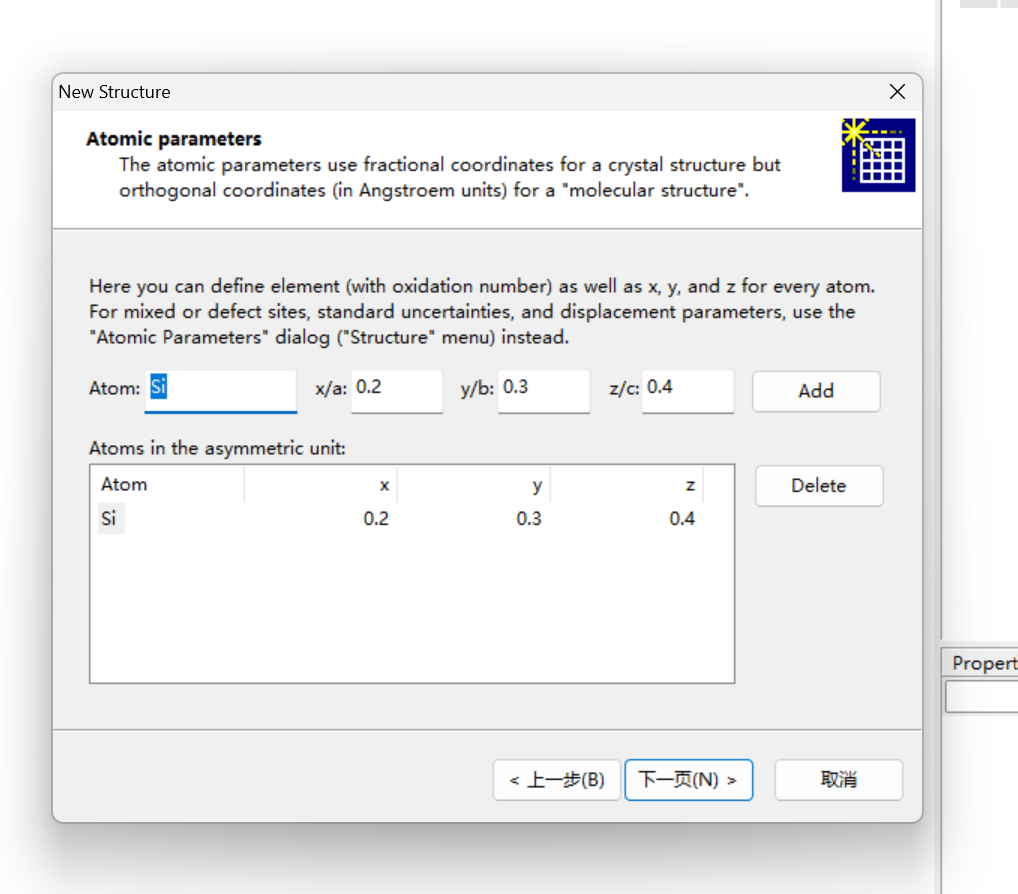
\includegraphics[width=0.44\textwidth]{assets/symmetry/inversion/b.png}}
  \caption{反演中心（$P\,\bar1$）演示的参数设置}
  \label{fig:sym-inv-param}
\end{figure}

\begin{figure}[H]
  \centering
  \subcaptionbox{(a) 单胞图：2 个原子关于反演中心等距反向}{%
    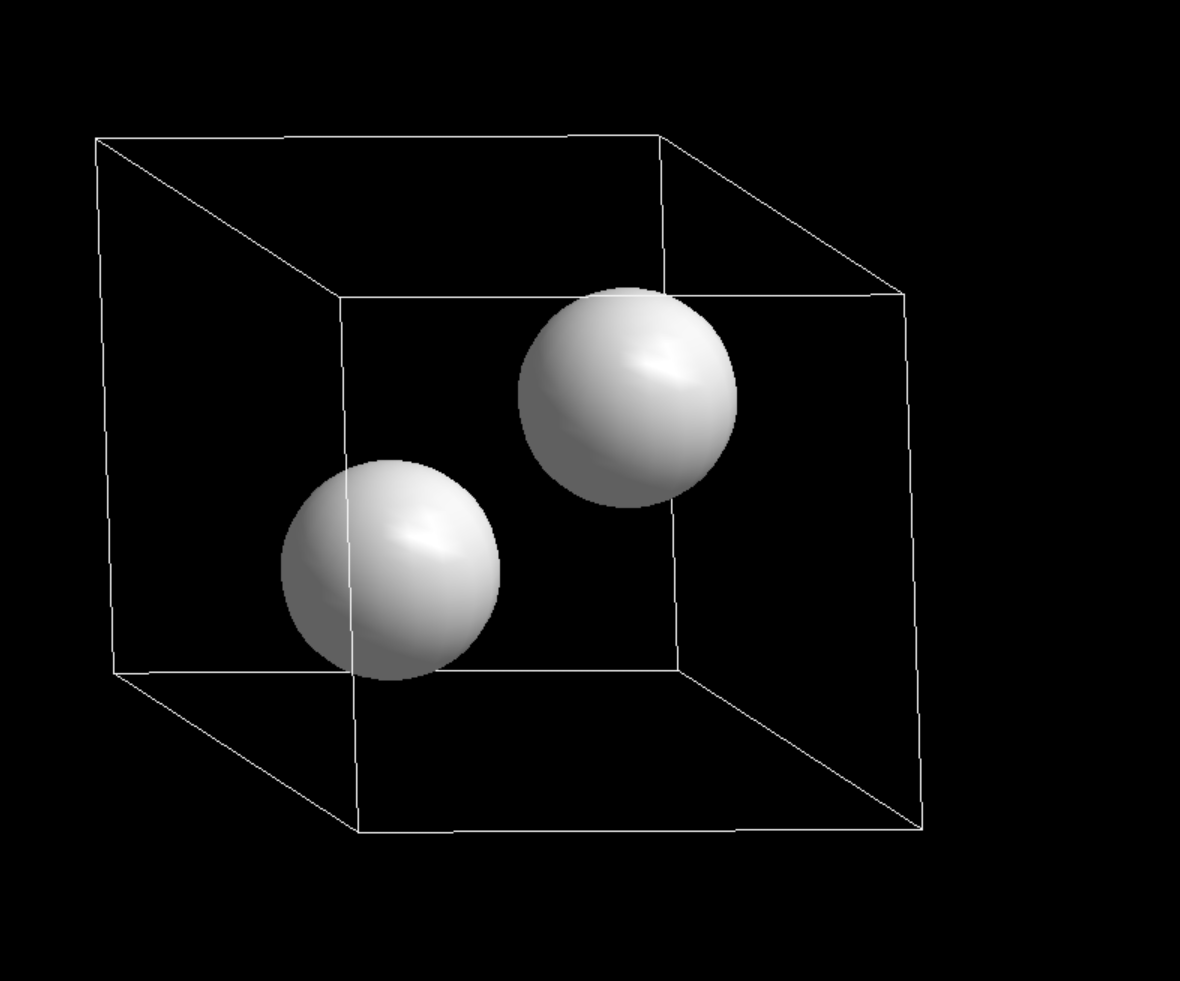
\includegraphics[width=0.44\textwidth]{assets/symmetry/inversion/c.png}}
  \hfill
  \subcaptionbox{(b) 超晶胞图：反演对在空间中的周期排列}{%
    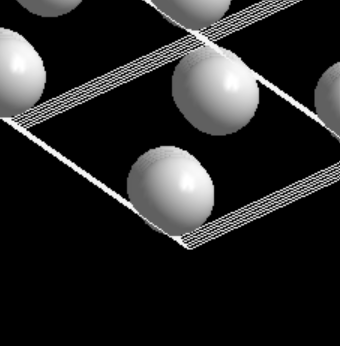
\includegraphics[width=0.44\textwidth]{assets/symmetry/inversion/d.png}}
  \caption{反演中心（$P\,\bar1$）的单胞与超晶胞模型}
  \label{fig:sym-inv-model}
\end{figure}

$P\,\bar1$ 的一般位置等效位置为 $(x,y,z)$ 与 $(\bar x,\bar y,\bar z)$，即全部原子都在
反演操作下``成对''出现：任意一个原子 $(x,y,z)$ 都存在一个与之关于原点等距反向的
配对原子。将 Si 的坐标 $(0.2,0.3,0.4)$ 代入，两个原子的分数坐标为
$(0.2,0.3,0.4)$ 与 $(0.8,0.7,0.6)$，分居晶胞体对角线的两端
（图~\ref{fig:sym-inv-model}(a)）；在超晶胞中，这些反演对沿三个方向周期重复
（图~\ref{fig:sym-inv-model}(b)）。

\textbf{特征与辨识要点。}反演操作的显著特征是``成对、共线、等距反向''：单胞内原子
数必为偶数（本例为 2），且每个原子都能找到一个关于中心等距反向的配对原子。作为
对照，若改用不含任何对称元素的 $P\,1$ 空间群输入同一坐标，晶胞内只会出现 1 个原子，
其位置不受任何对称约束——这正是 $P\,1$ 与 $P\,\bar1$ 两个符号的含义差别。反演
中心在衍射实验上也有明确后果：中心对称晶体的衍射强度严格满足 Friedel 定律
$I_{hkl}=I_{\bar h\bar k\bar l}$；当晶体不含反演中心时，在发生反常散射（波长接近
元素吸收边）的条件下会出现与 Friedel 定律的偏离，可据此辅助判断反演中心是否存在。
